\subsection{Model: Naïve Bayes}

\subsubsection{Introduction}

Naïve Bayes is a probabilistic classifier rooted in Bayes’ Theorem, making the (often simplifying) assumption that input features are conditionally independent given the class label. Despite its simplicity, Naïve Bayes can be very effective in text classification tasks by leveraging word frequencies or other vector representations. In this project, we used the GaussianNB variant to handle continuous input features such as TF-IDF and embedding vectors.

\subsubsection{Training Configuration}

The hyperparameter search space for GaussianNB was:

\begin{itemize}
    \item \textbf{Priors}: [\texttt{None}, [0.5, 0.5], [0.4, 0.6], [0.3, 0.7], [0.2, 0.8], [0.1, 0.9], [0.05, 0.95]]
    \item \textbf{Variance Smoothing} (\texttt{var\_smoothing}): \{1e-9, 1e-8, 1e-7\}
\end{itemize}

% We used K-Fold Cross-Validation to identify the best hyperparameter configuration based on Accuracy, with additional considerations for F1 score and ROC AUC. The final selected parameters were:

% \begin{itemize}
%     \item \textbf{Priors}: [0.3, 0.7]
%     \item \textbf{Variance Smoothing}: 1e-9
% \end{itemize}

A grid or random search was performed over these hyperparameters, employing K-Fold Cross-Validation to select the best configuration. The final chosen hyperparameters were validated on a withheld test set.

\subsubsection{Training and Evaluation Results}

The Naïve Bayes model was trained and evaluated using Count Vectorizer, TF-IDF, Word2Vec, and GloVe feature extraction. The tables below summarize the results for cross-validation (referred to as “Training”) and the final testing phase.

\textbf{Training Performance Metrics (Cross-Validation):}

\begin{table}[H]
    \centering
    \caption{Training Performance Metrics for Naïve Bayes (Cross-Validation Averages)}
    \label{tab:nb-training-metrics}
    \begin{tabular}{|l|c|c|c|c|c|}
        \hline
        \textbf{Method} & \textbf{Accuracy} & \textbf{ROC AUC} & \textbf{F1} & \textbf{Precision} & \textbf{Recall} \\ 
        \hline
        Count Vectorizer & 69\% & 69\% & 71\% & 69\% & 72\% \\ 
        \hline
        TF-IDF & 69\% & 69\% & 70\% & 69\% & 71\% \\ 
        \hline
        Word2Vec & 61\% & 61\% & 60\% & 64\% & 57\% \\ 
        \hline
        GloVe & 62\% & 62\% & 65\% & 62\% & 68\% \\ 
        \hline
    \end{tabular}
\end{table}

\textbf{Testing Performance Metrics:}

\begin{table}[H]
    \centering
    \caption{Testing Performance Metrics for Naïve Bayes}
    \label{tab:nb-testing-metrics}
    \begin{tabular}{|l|c|c|c|c|c|}
        \hline
        \textbf{Method} & \textbf{Accuracy} & \textbf{ROC AUC} & \textbf{F1} & \textbf{Precision} & \textbf{Recall} \\ 
        \hline
        Count Vectorizer & 0.7134 & 0.7463 & 0.7250 & 0.7151 & 0.7350 \\ 
        \hline
        TF-IDF & 0.7013 & 0.7357 & 0.7132 & 0.7038 & 0.7228 \\ 
        \hline
        Word2Vec & 0.6172 & 0.6743 & 0.6052 & 0.6438 & 0.5710 \\ 
        \hline
        GloVe & 0.6258 & 0.6704 & 0.6515 & 0.6246 & 0.6808 \\ 
        \hline
    \end{tabular}
\end{table}

\textbf{Best Model Selection Criteria:}

\begin{itemize}
    \item The best model is chosen based on testing performance, prioritizing Accuracy > F1 Score > ROC AUC.
    \item Under this criterion, the top-performing setup is:
\end{itemize}

\begin{verbatim}
{
    "method": "count",
    "model": "GaussianNB",
    "hyperparameters": {
        "priors": [0.3, 0.7],
        "var_smoothing": 1e-09
    },
    "performance": {
        "accuracy": 0.7134,
        "precision": 0.7151,
        "recall": 0.7350,
        "f1": 0.7250,
        "roc_auc": 0.7463491512402551
    }
}
\end{verbatim}

\subsubsection{Performance Analysis}

\begin{itemize}
    \item \textbf{Accuracy Analysis}: The highest accuracy (71.34\%) was achieved using Count Vectorizer, indicating that simpler bag-of-words features can be highly effective for Naïve Bayes in sentiment classification.
    \item \textbf{Probabilistic Modeling}: Specifying priors [0.3, 0.7] gave the best result, reflecting an optimal class balance assumption for the given dataset.
    \item \textbf{ROC AUC}: With a ROC AUC of 74.63\%, the model displayed adequate discrimination between positive and negative samples.
    \item \textbf{Precision and Recall}: Precision (71.51\%) and recall (73.50\%) are relatively balanced, suggesting Naïve Bayes handles both false positives and false negatives reasonably well.
    \item \textbf{Embedding Effects}: Word2Vec and GloVe yielded lower accuracies. This is likely because GaussianNB heavily relies on feature independence assumptions, which simpler Count/TF-IDF representations satisfy more closely than distributed embeddings.
\end{itemize}

\subsubsection{Visualization of Training Results}

The following figures illustrate the model’s performance across different embedding techniques:

\begin{figure}[H]
    \centering
    \begin{subfigure}[b]{0.48\textwidth}
        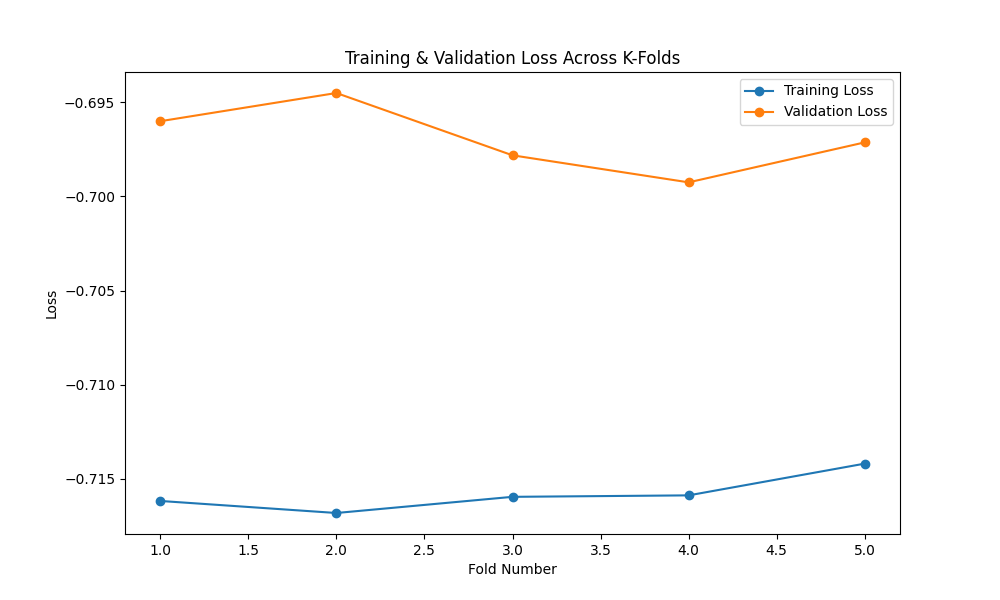
\includegraphics[width=\textwidth]{img/report_info/img/3.1.NaiveBayes/best_bayesian_count_loss.png}
        \caption{Loss Curve - Count Vectorizer}
        \label{fig:nb-count-loss}
    \end{subfigure}
    \begin{subfigure}[b]{0.48\textwidth}
        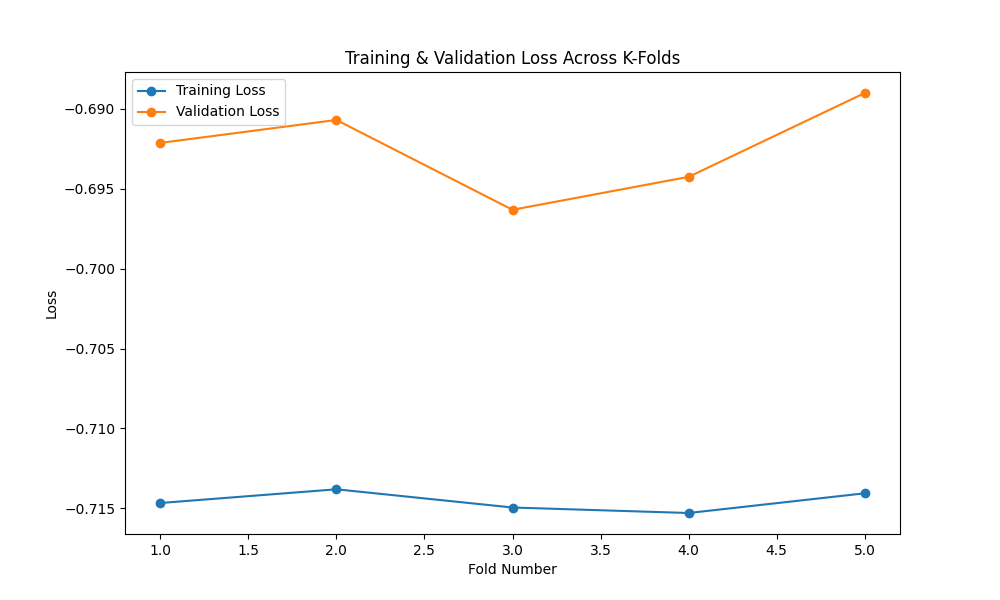
\includegraphics[width=\textwidth]{img/report_info/img/3.1.NaiveBayes/best_bayesian_tfidf_loss.png}
        \caption{Loss Curve - TF-IDF}
        \label{fig:nb-tfidf-loss}
    \end{subfigure}
    
    \begin{subfigure}[b]{0.48\textwidth}
        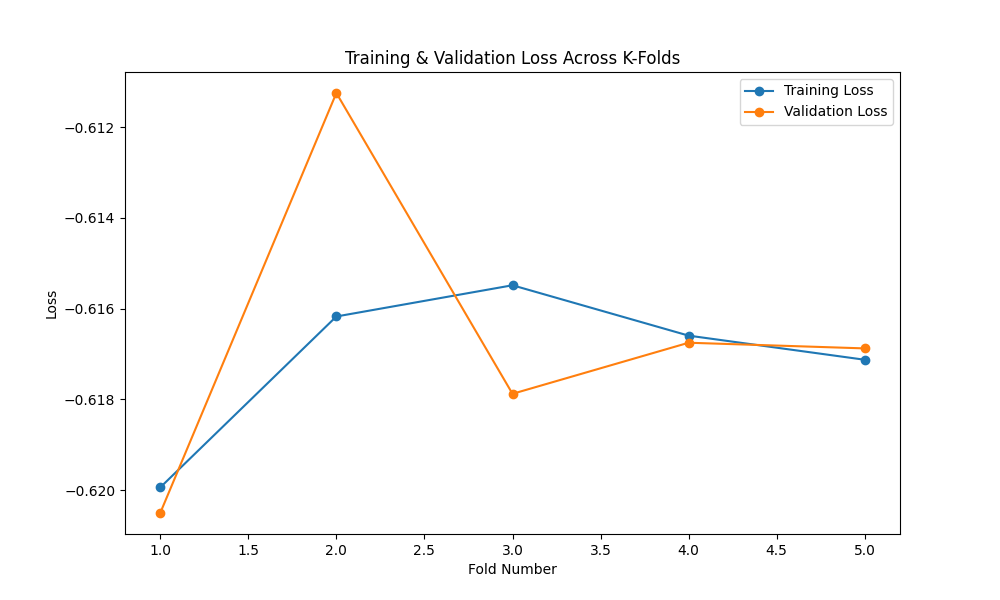
\includegraphics[width=\textwidth]{img/report_info/img/3.1.NaiveBayes/best_bayesian_word2vec_loss.png}
        \caption{Loss Curve - Word2Vec}
        \label{fig:nb-word2vec-loss}
    \end{subfigure}
    \begin{subfigure}[b]{0.48\textwidth}
        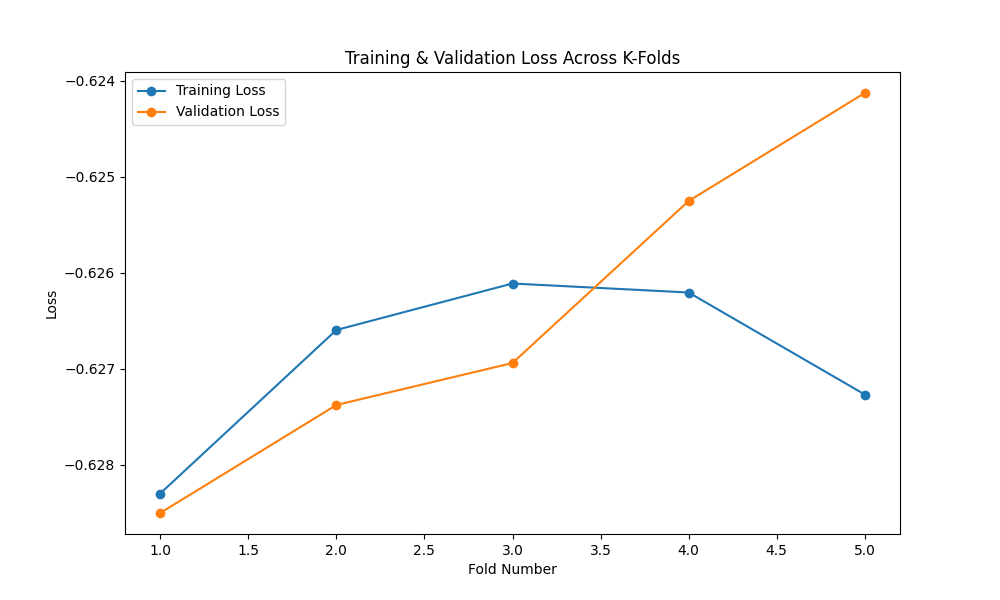
\includegraphics[width=\textwidth]{img/report_info/img/3.1.NaiveBayes/best_bayesian_glove_loss.png}
        \caption{Loss Curve - GloVe}
        \label{fig:nb-glove-loss}
    \end{subfigure}
    
    \caption{Comparison of Loss Curves for Naïve Bayes across Different Feature Extraction Methods}
    \label{fig:nb-loss-group}
\end{figure}

\begin{figure}[H]
    \centering
    \begin{subfigure}[b]{0.48\textwidth}
        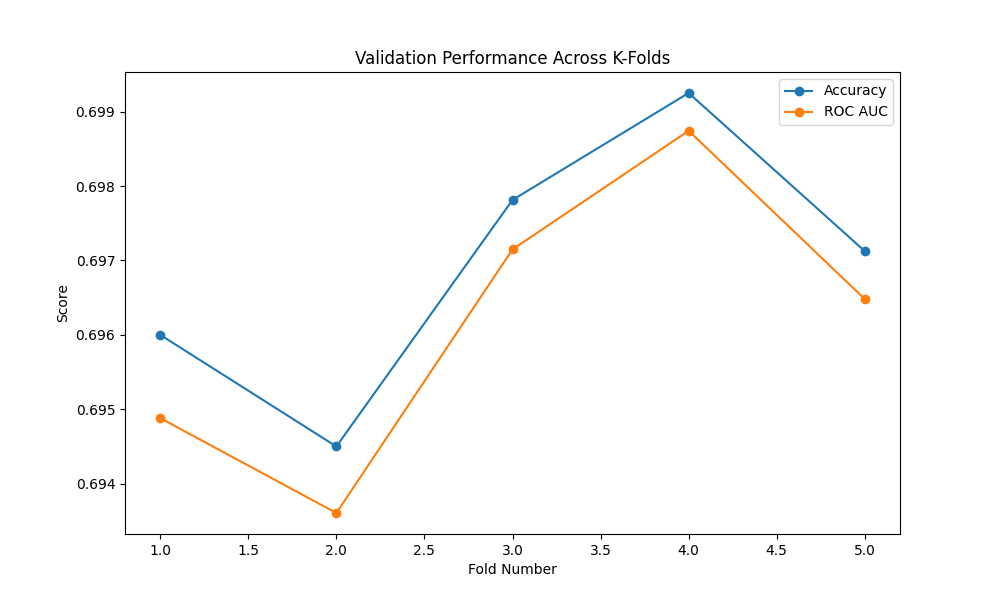
\includegraphics[width=\textwidth]{img/report_info/img/3.1.NaiveBayes/best_bayesian_count.png}
        \caption{Performance - Count Vectorizer}
        \label{fig:nb-count}
    \end{subfigure}
    \begin{subfigure}[b]{0.48\textwidth}
        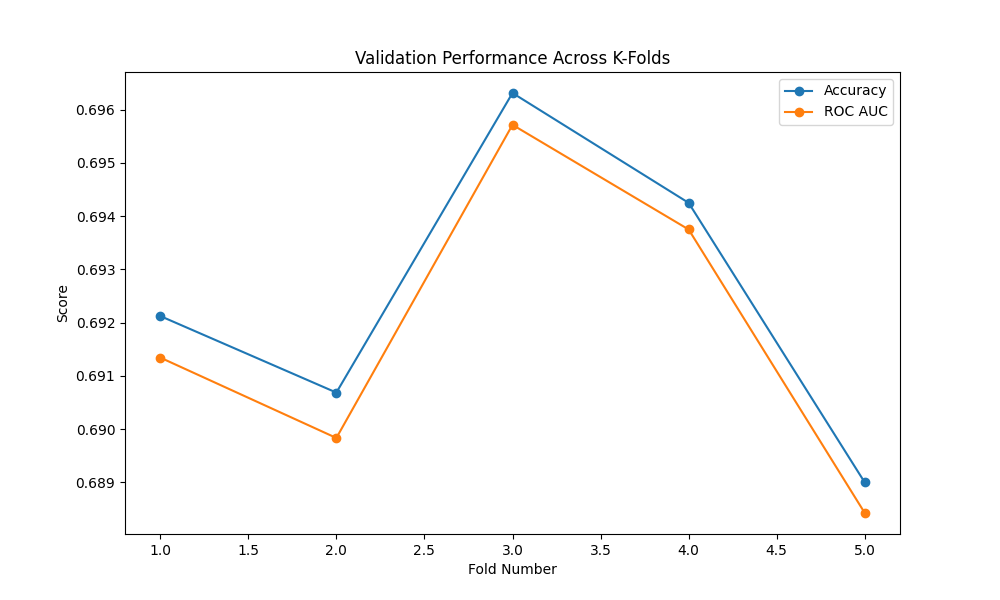
\includegraphics[width=\textwidth]{img/report_info/img/3.1.NaiveBayes/best_bayesian_tfidf.png}
        \caption{Performance - TF-IDF}
        \label{fig:nb-tfidf}
    \end{subfigure}
    
    \begin{subfigure}[b]{0.48\textwidth}
        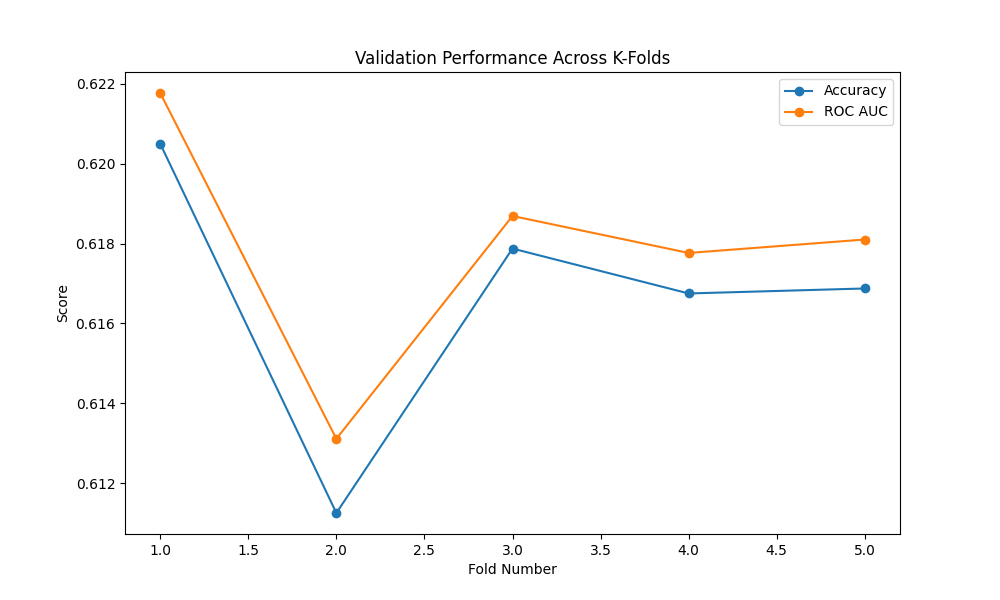
\includegraphics[width=\textwidth]{img/report_info/img/3.1.NaiveBayes/best_bayesian_word2vec.png}
        \caption{Performance - Word2Vec}
        \label{fig:nb-word2vec}
    \end{subfigure}
    \begin{subfigure}[b]{0.48\textwidth}
        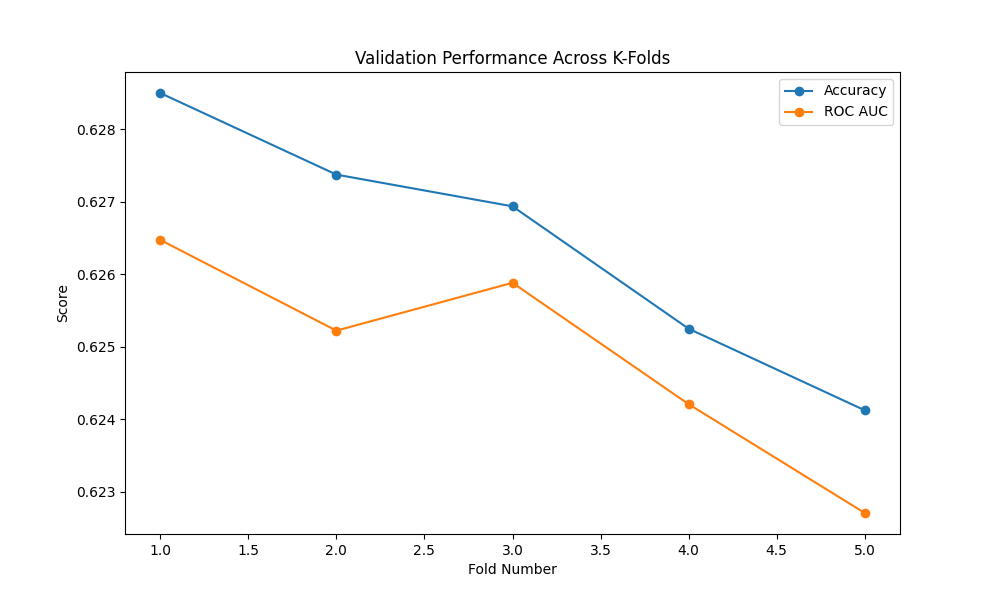
\includegraphics[width=\textwidth]{img/report_info/img/3.1.NaiveBayes/best_bayesian_glove.png}
        \caption{Performance - GloVe}
        \label{fig:nb-glove}
    \end{subfigure}
    
    \caption{Comparison of Training Performance Metrics for Naïve Bayes across Different Feature Extraction Methods}
    \label{fig:nb-performance-group}
\end{figure}

\textbf{Image Description:}

\begin{itemize}
    \item \textbf{Training and Validation Loss Analysis:}
    \begin{itemize}
        \item Loss curves remain generally stable, though the inherent assumption of feature independence in Naïve Bayes can cause volatility if embeddings have correlated dimensions.
        \item Count Vectorizer and TF-IDF tend to exhibit less fluctuation compared to Word2Vec and GloVe.
    \end{itemize}
    
    \item \textbf{Validation Performance Metrics:}
    \begin{itemize}
        \item Count Vectorizer shows the highest and most consistent accuracy and F1 scores, mirroring the final model selection.
        \item TF-IDF’s performance is a close second, with slight variations across folds.
        \item Word2Vec and GloVe produce more variable outcomes, reflecting less synergy with GaussianNB’s simplified assumptions.
    \end{itemize}
\end{itemize}

\subsubsection{Computational Resources and Efficiency}

Naïve Bayes is a computationally lightweight model, making it highly efficient in terms of training time and resource consumption. Given the dataset size of 500,000 samples, we estimate the following computational costs:

\begin{itemize}
    \item \textbf{Training Time:} Less than 5 minutes on a modern CPU (Intel Core i7-12700K or equivalent) since Naïve Bayes only requires a single pass over the data to estimate probabilities.
    \item \textbf{Memory Usage:} Approximately 1-2GB RAM during training, depending on the feature extraction method.
    \begin{itemize}
        \item \textbf{Count Vectorizer / TF-IDF:} Requires around 1GB RAM for matrix storage and computations.
        \item \textbf{Word2Vec / GloVe:} Can require up to 2GB RAM due to the dense nature of word embeddings.
    \end{itemize}
    \item \textbf{Inference Speed:} Extremely fast, taking less than 1 millisecond per sample, making it suitable for real-time applications.
    \item \textbf{Disk Space:} The trained model file size is relatively small, typically under 50MB when storing probability tables.
\end{itemize}

Due to its low computational cost, Naïve Bayes is an excellent choice for large-scale text classification tasks where training and inference speed are critical.

\subsubsection{Conclusion}

Naïve Bayes (GaussianNB) proved effective for sentiment classification when coupled with Count Vectorizer features, achieving a 71.34\% accuracy. The class priors [0.3, 0.7] suggest that accommodating class imbalance can be beneficial for this dataset. While TF-IDF also delivered competitive results, the simpler bag-of-words representation ultimately offered the best balance of accuracy and F1 performance for Naïve Bayes in this study.

\newpage